% auto-generated by v10_maketikz.m
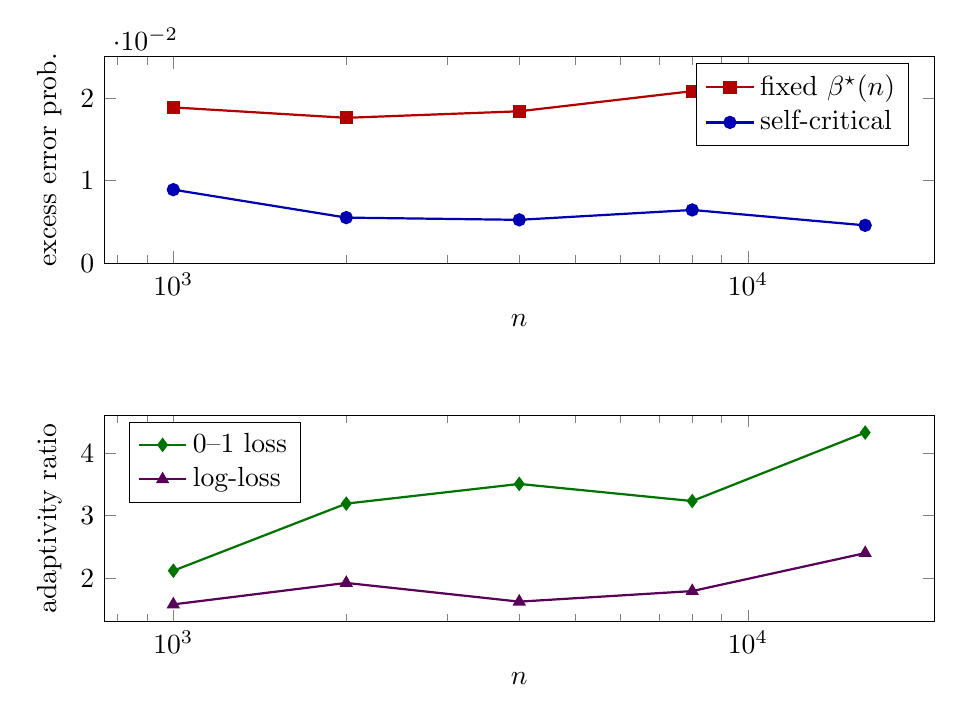
\begin{tikzpicture}
\begin{semilogxaxis}[name=bx1,width=\linewidth,height=4.2cm,
  xlabel={$n$},ylabel={excess error prob.},ymin=0,ymax=0.025,
  legend pos=north east,legend cell align=left,
  every axis plot/.append style={thick}]
\addplot[mark=square*,red!70!black] coordinates {(1000,0.018882) (2000,0.017618) (4000,0.018409) (8000,0.02085) (16000,0.019827) };
\addplot[mark=*,blue!70!black] coordinates {(1000,0.0089067) (2000,0.0055166) (4000,0.0052471) (8000,0.0064461) (16000,0.0045789) };
\legend{fixed $\beta^\star(n)$,self-critical}
\end{semilogxaxis}
\begin{semilogxaxis}[name=bx2,at={(bx1.below south west)},anchor=above north west,yshift=-1.0cm,
  width=\linewidth,height=4.2cm,
  xlabel={$n$},ylabel={adaptivity ratio},
  legend pos=north west,legend cell align=left,
  every axis plot/.append style={thick}]
\addplot[mark=diamond*,green!45!black] coordinates {(1000,2.12) (2000,3.1935) (4000,3.5085) (8000,3.2345) (16000,4.3301) };
\addplot[mark=triangle*,violet!70!black] coordinates {(1000,1.581) (2000,1.9247) (4000,1.6252) (8000,1.7941) (16000,2.4017) };
\legend{0--1 loss,log-loss}
\end{semilogxaxis}
\end{tikzpicture}
